\chapter{Introdução}

\section{Propósito}
Desenvolvimento de um programa distribuído que possibilite a realização de disputas do jogo
``\gls{alapo}''\cite{alapoWebsite} na modalidade
\textit{usuário vs.\ usuário}.

\section{Regras do jogo}\label{section:regras}
O jogo deve ser jogado em um tabuleiro quadrado de 36 ($6 \times 6$) posições; cada jogador deve iniciar uma partida com
12 peças para si, para um total de 24 peças no tabuleiro no momento que a partida é iniciada.\\
As peças do jogo são de seis (6) tipos diferentes, e cada jogador deve receber duas peças de cada tipo, sendo que as
peças devem ser identificadas por cor, para que se possa fazer a distinção entre quais peças no tabuleiro pertencem a
cada jogador:

\begin{description}
  \item [Peça Triangular Grande:] \hfill\\ Sinalizada neste documento pelo símbolo ``\gls{bbt}'', o movimento dessa
    peça é oblíquo, ou seja, pode movimentar-se diagonalmente no tabuleiro, e pode fazê-lo por quantas posições o
    jogador desejar; \textbf{\textit{duas peças para cada jogador}};
  \item [Peça Quadrada Grande:] \hfill\\ Sinalizada neste documento pelo símbolo ``\gls{bbs}'', o movimento dessa peça
    é ortogonal, ou seja, pode movimentar-se horizontalmente como verticalmente no tabuleiro, e pode fazê-lo por
    quantas posições o jogador desejar; \textbf{\textit{duas peças para cada jogador}};
  \item [Peça Circular Grande:] \hfill\\ Sinalizada neste documento pelo símbolo ``\gls{bbc}''; o movimento dessa peça
    abrange manobras diagonais assim como ortogonais, podendo ser movida em todas as direções, por quantas posições o
    jogador desejar; \textbf{\textit{duas peças para cada jogador}};
  \item [Peça Triangular Pequena:] \hfill\\ Sinalizada neste documento pelo símbolo ``\gls{sbt}''; o movimento dessa
    peça é oblíquo, ou seja, pode movimentar-se diagonalmente no tabuleiro, porém apenas uma por posição por vez;
    \textbf{\textit{duas peças para cada jogador}};
  \item [Peça Quadrada Pequena:] \hfill\\ Sinalizada neste documento pelo símbolo ``\gls{sbs}''; o movimento dessa
    peça é ortogonal, ou seja, pode movimentar-se horizontalmente como verticalmente no tabuleiro, porém apenas uma
    por posição por vez; \textbf{\textit{duas peças para cada jogador}};
  \item [Peça Circular Pequena:] \hfill\\ Sinalizada neste documento pelo símbolo ``\gls{sbc}''; o movimento dessa
    peça abrange manobras diagonais assim como ortogonais, podendo ser movida em todas as direções, porém apenas uma
    por posição por vez; \textbf{\textit{duas peças para cada jogador}};
\end{description}

\subsection{Sobre a movimentação}
\begin{itemize}
  \item A movimentação do jogo \textbf{não permite} que peças ``pulem'' por cima umas das outras, ou seja, as peças só
    podem transitar por um trecho que está inobstruído do início ao fim;
  \item O jogo é jogado em turnos; cada jogador deve realizar \textbf{apenas um movimento por turno};
  \item A \textit{captura} é realizada ao passar uma peça para a posição onde uma peça do oponente está ocupando
    (análogo à forma que essa mecânica se apresenta no \textit{xadrez} ou na \textit{dama});
\end{itemize}

\newpage

\subsection{Configuração inicial do tabuleiro}
Para começar uma partida as peças devem ser posicionadas, em extremidades do tabuleiro, por cada jogador, na seguinte
disposição:

\begin{itemize}
  \item As peças \textbf{maiores} (\gls{bbt}, \gls{bbs}, \gls{bbc}) devem ser posicionadas ao longo da \textbf{primeira linha} relativa
    ao jogador (linha ``1'' ou linha ``6'', dependendo da perspectiva);
  \item As peças \textbf{menores} (\gls{sbt}, \gls{sbs}, \gls{sbc}) devem ser posicionadas ao longo da \textbf{segunda linha} relativa
    ao jogador (linha ``2'' ou linha ``5'', dependendo da perspectiva);
  \item As peças \textbf{quadradas} (\gls{bbs}, \gls{sbs}) devem ser posicionadas nas posições pertencentes às colunas mais
    externas do tabuleiro (colunas ``$A$'' e ``$F$'');
  \item As peças \textbf{triangulares} (\gls{bbt}, \gls{sbt}) devem ser posicionadas nas posições imediatamente interas às peças
    \textbf{quadradas} (colunas ``$B$'' e ``$E$'');
  \item As peças \textbf{circulares} (\gls{bbc}, \gls{sbc}) devem ser posicionadas nas posições pertencentes às colunas mais
    internas do tabuleiro (colunas ``$C$'' e ``$D$'');
\end{itemize}
De maneira que o tabuleiro apresente a seguinte configuração, assim que todas as peças estejam devidamente posicionadas:

\begin{figure}[h]
    \centering
    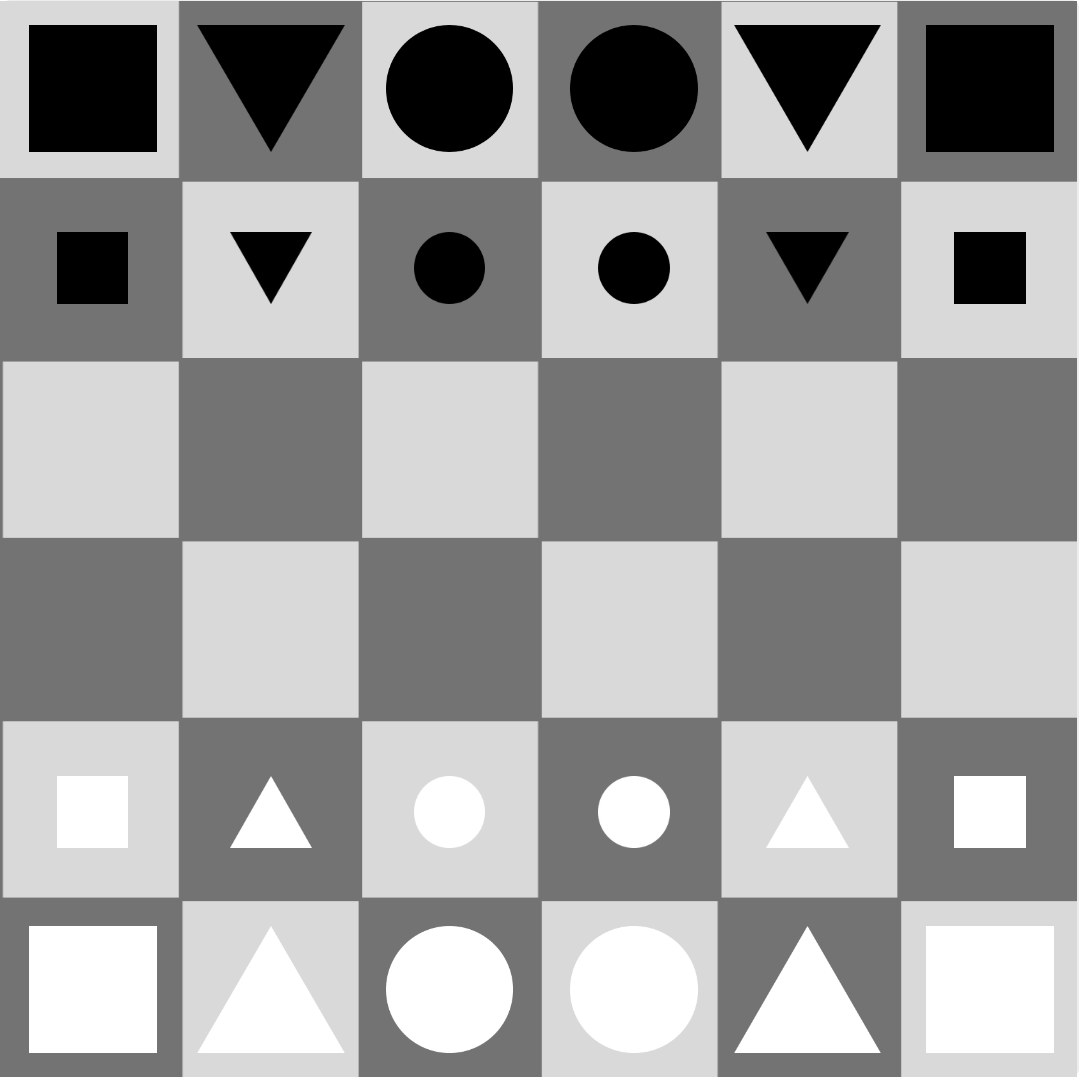
\includegraphics[width=10cm]{Images/figure_1_board_setup}
    \caption{Configuração inicial do tabuleiro}
    \label{fig:configuracao tabuleiro}
\end{figure}

\subsection{Progressão da partida}\label{section:progressao}
Assim que as peças estiverem posicionadas, um dos jogadores (qual jogador iniciará a primeira jogada pode ser escolhido
aleatoriamente) escolhe uma das suas peças e faz o primeiro movimento. Os jogadores tomam turnos realizando lances
(movimentos) e capturando as peças um do outro, com o objetivo alcançar a extremidade oposta do tabuleiro com uma de suas
peças, sem ser capturado.

\begin{itemize}
  \item Uma \textbf{vitória} é configurada quando um jogador alcança o extremo oposto do tabuleiro \textit{sem ter sua
    posição imediatamente contestada}, isto é, quando a posição ocupada pela peça não está a alcance de captura de
    nenhuma peça do oponente;
  \item Um \textbf{empate} é configurado quando a condição de vitória é alcançada por ambos os jogadores no \textit{no
    intervalo de um turno};
  \item Caso um jogador alcance o extremo oposto do tabuleiro e a posição ocupada pela peça seja contestável pelo
    oponente, \textbf{a contestação por parte do oponente é obrigatória} e deve ser realizada no turno imediatamente
    após a ocupação da posição;
\end{itemize}

